% Options for packages loaded elsewhere
\PassOptionsToPackage{unicode}{hyperref}
\PassOptionsToPackage{hyphens}{url}
%
\documentclass[
  12pt,
  norsk,
]{article}
\usepackage{amsmath,amssymb}
\usepackage{lmodern}
\usepackage{ifxetex,ifluatex}
\ifnum 0\ifxetex 1\fi\ifluatex 1\fi=0 % if pdftex
  \usepackage[T1]{fontenc}
  \usepackage[utf8]{inputenc}
  \usepackage{textcomp} % provide euro and other symbols
\else % if luatex or xetex
  \usepackage{unicode-math}
  \defaultfontfeatures{Scale=MatchLowercase}
  \defaultfontfeatures[\rmfamily]{Ligatures=TeX,Scale=1}
\fi
% Use upquote if available, for straight quotes in verbatim environments
\IfFileExists{upquote.sty}{\usepackage{upquote}}{}
\IfFileExists{microtype.sty}{% use microtype if available
  \usepackage[]{microtype}
  \UseMicrotypeSet[protrusion]{basicmath} % disable protrusion for tt fonts
}{}
\makeatletter
\@ifundefined{KOMAClassName}{% if non-KOMA class
  \IfFileExists{parskip.sty}{%
    \usepackage{parskip}
  }{% else
    \setlength{\parindent}{0pt}
    \setlength{\parskip}{6pt plus 2pt minus 1pt}}
}{% if KOMA class
  \KOMAoptions{parskip=half}}
\makeatother
\usepackage{xcolor}
\IfFileExists{xurl.sty}{\usepackage{xurl}}{} % add URL line breaks if available
\IfFileExists{bookmark.sty}{\usepackage{bookmark}}{\usepackage{hyperref}}
\hypersetup{
  pdftitle={Er det høyde som bestemmer inntekt?},
  pdfauthor={Assignment 2 i kurset Data Science 2021 - Karoline Midtbø og Morten Knutsen},
  pdflang={nb-NO},
  hidelinks,
  pdfcreator={LaTeX via pandoc}}
\urlstyle{same} % disable monospaced font for URLs
\usepackage[margin=1in]{geometry}
\usepackage{color}
\usepackage{fancyvrb}
\newcommand{\VerbBar}{|}
\newcommand{\VERB}{\Verb[commandchars=\\\{\}]}
\DefineVerbatimEnvironment{Highlighting}{Verbatim}{commandchars=\\\{\}}
% Add ',fontsize=\small' for more characters per line
\usepackage{framed}
\definecolor{shadecolor}{RGB}{248,248,248}
\newenvironment{Shaded}{\begin{snugshade}}{\end{snugshade}}
\newcommand{\AlertTok}[1]{\textcolor[rgb]{0.94,0.16,0.16}{#1}}
\newcommand{\AnnotationTok}[1]{\textcolor[rgb]{0.56,0.35,0.01}{\textbf{\textit{#1}}}}
\newcommand{\AttributeTok}[1]{\textcolor[rgb]{0.77,0.63,0.00}{#1}}
\newcommand{\BaseNTok}[1]{\textcolor[rgb]{0.00,0.00,0.81}{#1}}
\newcommand{\BuiltInTok}[1]{#1}
\newcommand{\CharTok}[1]{\textcolor[rgb]{0.31,0.60,0.02}{#1}}
\newcommand{\CommentTok}[1]{\textcolor[rgb]{0.56,0.35,0.01}{\textit{#1}}}
\newcommand{\CommentVarTok}[1]{\textcolor[rgb]{0.56,0.35,0.01}{\textbf{\textit{#1}}}}
\newcommand{\ConstantTok}[1]{\textcolor[rgb]{0.00,0.00,0.00}{#1}}
\newcommand{\ControlFlowTok}[1]{\textcolor[rgb]{0.13,0.29,0.53}{\textbf{#1}}}
\newcommand{\DataTypeTok}[1]{\textcolor[rgb]{0.13,0.29,0.53}{#1}}
\newcommand{\DecValTok}[1]{\textcolor[rgb]{0.00,0.00,0.81}{#1}}
\newcommand{\DocumentationTok}[1]{\textcolor[rgb]{0.56,0.35,0.01}{\textbf{\textit{#1}}}}
\newcommand{\ErrorTok}[1]{\textcolor[rgb]{0.64,0.00,0.00}{\textbf{#1}}}
\newcommand{\ExtensionTok}[1]{#1}
\newcommand{\FloatTok}[1]{\textcolor[rgb]{0.00,0.00,0.81}{#1}}
\newcommand{\FunctionTok}[1]{\textcolor[rgb]{0.00,0.00,0.00}{#1}}
\newcommand{\ImportTok}[1]{#1}
\newcommand{\InformationTok}[1]{\textcolor[rgb]{0.56,0.35,0.01}{\textbf{\textit{#1}}}}
\newcommand{\KeywordTok}[1]{\textcolor[rgb]{0.13,0.29,0.53}{\textbf{#1}}}
\newcommand{\NormalTok}[1]{#1}
\newcommand{\OperatorTok}[1]{\textcolor[rgb]{0.81,0.36,0.00}{\textbf{#1}}}
\newcommand{\OtherTok}[1]{\textcolor[rgb]{0.56,0.35,0.01}{#1}}
\newcommand{\PreprocessorTok}[1]{\textcolor[rgb]{0.56,0.35,0.01}{\textit{#1}}}
\newcommand{\RegionMarkerTok}[1]{#1}
\newcommand{\SpecialCharTok}[1]{\textcolor[rgb]{0.00,0.00,0.00}{#1}}
\newcommand{\SpecialStringTok}[1]{\textcolor[rgb]{0.31,0.60,0.02}{#1}}
\newcommand{\StringTok}[1]{\textcolor[rgb]{0.31,0.60,0.02}{#1}}
\newcommand{\VariableTok}[1]{\textcolor[rgb]{0.00,0.00,0.00}{#1}}
\newcommand{\VerbatimStringTok}[1]{\textcolor[rgb]{0.31,0.60,0.02}{#1}}
\newcommand{\WarningTok}[1]{\textcolor[rgb]{0.56,0.35,0.01}{\textbf{\textit{#1}}}}
\usepackage{graphicx}
\makeatletter
\def\maxwidth{\ifdim\Gin@nat@width>\linewidth\linewidth\else\Gin@nat@width\fi}
\def\maxheight{\ifdim\Gin@nat@height>\textheight\textheight\else\Gin@nat@height\fi}
\makeatother
% Scale images if necessary, so that they will not overflow the page
% margins by default, and it is still possible to overwrite the defaults
% using explicit options in \includegraphics[width, height, ...]{}
\setkeys{Gin}{width=\maxwidth,height=\maxheight,keepaspectratio}
% Set default figure placement to htbp
\makeatletter
\def\fps@figure{htbp}
\makeatother
\setlength{\emergencystretch}{3em} % prevent overfull lines
\providecommand{\tightlist}{%
  \setlength{\itemsep}{0pt}\setlength{\parskip}{0pt}}
\setcounter{secnumdepth}{-\maxdimen} % remove section numbering
\usepackage{array}
\usepackage{caption}
\usepackage{graphicx}
\usepackage{siunitx}
\usepackage[normalem]{ulem}
\usepackage{colortbl}
\usepackage{multirow}
\usepackage{hhline}
\usepackage{calc}
\usepackage{tabularx}
\usepackage{threeparttable}
\usepackage{wrapfig}
\usepackage{adjustbox}
\usepackage{hyperref}
\ifxetex
  % Load polyglossia as late as possible: uses bidi with RTL langages (e.g. Hebrew, Arabic)
  \usepackage{polyglossia}
  \setmainlanguage[]{norsk}
\else
  \usepackage[main=norsk]{babel}
% get rid of language-specific shorthands (see #6817):
\let\LanguageShortHands\languageshorthands
\def\languageshorthands#1{}
\fi
\ifluatex
  \usepackage{selnolig}  % disable illegal ligatures
\fi

\title{Er det høyde som bestemmer inntekt?}
\author{Assignment 2 i kurset Data Science 2021 - Karoline Midtbø og
Morten Knutsen}
\date{}

\begin{document}
\maketitle

\begin{Shaded}
\begin{Highlighting}[]
\FunctionTok{library}\NormalTok{(modelr)}
\FunctionTok{library}\NormalTok{(ggplot2)}
\FunctionTok{library}\NormalTok{(tinytex)}
\FunctionTok{library}\NormalTok{(tidyverse)}
\end{Highlighting}
\end{Shaded}

\begin{verbatim}
## -- Attaching packages --------------------------------------- tidyverse 1.3.1 --
\end{verbatim}

\begin{verbatim}
## v tibble  3.1.3     v dplyr   1.0.7
## v tidyr   1.1.3     v stringr 1.4.0
## v readr   2.0.1     v forcats 0.5.1
## v purrr   0.3.4
\end{verbatim}

\begin{verbatim}
## -- Conflicts ------------------------------------------ tidyverse_conflicts() --
## x dplyr::filter() masks stats::filter()
## x dplyr::lag()    masks stats::lag()
\end{verbatim}

\begin{Shaded}
\begin{Highlighting}[]
\FunctionTok{library}\NormalTok{(ggpubr)}
\FunctionTok{library}\NormalTok{(huxtable)}
\end{Highlighting}
\end{Shaded}

\begin{verbatim}
## 
## Attaching package: 'huxtable'
\end{verbatim}

\begin{verbatim}
## The following object is masked from 'package:ggpubr':
## 
##     font
\end{verbatim}

\begin{verbatim}
## The following object is masked from 'package:dplyr':
## 
##     add_rownames
\end{verbatim}

\begin{verbatim}
## The following object is masked from 'package:ggplot2':
## 
##     theme_grey
\end{verbatim}

\begin{Shaded}
\begin{Highlighting}[]
\FunctionTok{library}\NormalTok{(car)}
\end{Highlighting}
\end{Shaded}

\begin{verbatim}
## Loading required package: carData
\end{verbatim}

\begin{verbatim}
## 
## Attaching package: 'car'
\end{verbatim}

\begin{verbatim}
## The following object is masked from 'package:dplyr':
## 
##     recode
\end{verbatim}

\begin{verbatim}
## The following object is masked from 'package:purrr':
## 
##     some
\end{verbatim}

\begin{Shaded}
\begin{Highlighting}[]
\FunctionTok{library}\NormalTok{(carData)}
\FunctionTok{options}\NormalTok{(}\AttributeTok{scipen =} \DecValTok{999}\NormalTok{)}
\end{Highlighting}
\end{Shaded}

\#Er det høyde som bestemmer inntekt?

\hypertarget{i-denne-artikkelen-skal-vi-skrive-om-det-er-huxf8yden-som-puxe5virker-inntekten.-vi-har-sett-puxe5-to-ulike-kilder-som-viser-til-ulike-studier-om-hvordan-huxf8yd-epuxe5virker-inntekt.-der-det-ufuxf8res-ulike-undersuxf8kelser-for-uxe5-finne-ut-om-sannheten-om-at-huxf8yden-spiller-en-rolle-nuxe5r-det-kommer-til-huxf8yde.-vi-skal-ogsuxe5-utfuxf8re-ulike-datasett-der-vi-selv-ser-puxe5-hvordan-huxf8yde-puxe5virker-inntekt-ved-bruk-av-ulike-dataer.-til-slutt-skal-vi-komme-frem-til-en-konklusjon-og-presentere-vuxe5rt-svar-puxe5-spuxf8rsmuxe5let.}{%
\section{I denne artikkelen skal vi skrive om det er høyden som påvirker
inntekten. Vi har sett på to ulike kilder som viser til ulike studier om
hvordan høyd epåvirker inntekt. Der det uføres ulike undersøkelser for å
finne ut om sannheten om at høyden spiller en rolle når det kommer til
høyde. Vi skal også utføre ulike datasett der vi selv ser på hvordan
høyde påvirker inntekt, ved bruk av ulike dataer. Til slutt skal vi
komme frem til en konklusjon og presentere vårt svar på
spørsmålet.}\label{i-denne-artikkelen-skal-vi-skrive-om-det-er-huxf8yden-som-puxe5virker-inntekten.-vi-har-sett-puxe5-to-ulike-kilder-som-viser-til-ulike-studier-om-hvordan-huxf8yd-epuxe5virker-inntekt.-der-det-ufuxf8res-ulike-undersuxf8kelser-for-uxe5-finne-ut-om-sannheten-om-at-huxf8yden-spiller-en-rolle-nuxe5r-det-kommer-til-huxf8yde.-vi-skal-ogsuxe5-utfuxf8re-ulike-datasett-der-vi-selv-ser-puxe5-hvordan-huxf8yde-puxe5virker-inntekt-ved-bruk-av-ulike-dataer.-til-slutt-skal-vi-komme-frem-til-en-konklusjon-og-presentere-vuxe5rt-svar-puxe5-spuxf8rsmuxe5let.}}

Her tar vi å gjør om til målenhetene til metriske. Vi har også lagt til
tre nye variabler.

\hypertarget{litteraturgjennomgang}{%
\subsection{Litteraturgjennomgang}\label{litteraturgjennomgang}}

I 2004 skrev Judge og Cable en artikkel der de inkluderte en analyse på
om høyde påvirker inntekt. De utførte en analyse med flere
kontrollvariabler. De kontrollvariablene var kjønn, alder, vekt og
metode. I følge artikkelen kan kjønn ha en påvirkning på både høyde og
inntekt. Innen høyde vil de si at gjennomsnittet på høyde på menn og
kvinner har en forskjell. I Amerika er gjennomsnittet på menn på 175,5
og på kvinner er 161,7 som tilvarer en forskjell på
12,7(\protect\hyperlink{ref-JudgeCabel2004}{\textbf{JudgeCabel2004?}}).
Når det kommer til alder, vil mennesker i gjennomsnitt minske 5 cm i
løpet av levetiden. Høyde og vekt er tydligvis korrelerte, men kan
alikevell ha effekter i motsatte retninger, de bør derfor isolers og
behandles hver for seg i en analyse. Den siste kontrollvariablene er
metode der det vises til at det skal undersøkes på tvers av fire
komplementære prøver. De begrenset analysene til personer som hadde et
gjennomsnitt på 20 timer eller mer arbeid per uke, bortsett fra studie
1, der vi begrenset analysene til enkeltpersoner som var de primære
lønnstakerne i familien.

Studie 1 gikk ut på deltakere og prosedyre der de samlet inn alder,
kjønn, høyde og vekt.I studiet 2 samlet de inn lønn, alder, kjønn, høyde
og vekt fra en kilde. I studiet 3 samlet de samme data som i studiet 2
men bare i en ny kilde. I siste studiet fra en siste kilde. Resultatene
de fikk av dette var at i alle studiene var høyden signifikant positivt
korrelert med inntjeningen. I studie 1 viser regresjonsresultatene at
alder forutsier positivt inntjening. For studie 2 forutsier kjønn
negativ inntjening slik at kvinner tjener mindre enn menn. Alder
forutsier positivt inntjening og vekt forutsier negativt inntjening. For
studie 3 forutsier høyden betydelig inntjening. Til slutt, i studie 4,
forutsier hver inntekt betydelig. Multippelkorrelasjonen er R = .29, og
de uavhengige variablene forklarer 8\% av variansen i inntjening. Ved å
beregne gjennomsnittet på tvers av disse resultatene, finner vi ut at en
person som er 72 tommer høy kan forventes å tjene 5.525 dollar mer per
år enn noen som er 65 tommer høy, selv etter å ha kontrollert kjønn,
vekt og alder.

I en annen artikkel skrevet av Deaton og Arora ble det brukt data fra
Gallup-Healthways Well-Being Index, der de hadde daglige meningsmåling
om å undersøke forholdet mellom høyde og en rekke emosjonelle og
evaluerende utfall. De ser på 454 065 voksne i alderen 18 år eller eldre
som ble intervjuet fra 2. januar 2008 til 16. april 2009. De ble da
spørt om høyde og ble bedt om å plasere livssituasjon i en rank fra 0
til 10, der 0 fra ``det verste mulige liv for deg'' og 10 var ``det best
mulige livet for deg''. De bes også om å svare ja eller nei på spørsmål
om følelsene de har hatt i løpet av dagen. Menn som er over
gjennomsnittlig høyde rapporterer at de er litt mer enn en sjuendedel av
trinnet på ranken over menn som er under gjennomsnittlig høyde,
gjennomsnittlig poengsum på 6,55 mot 6,41. For kvinner er forskjellen
mindre, med kvinner under gjennomsnittlig høyd litt mindre enn en
tiendedel av ranken under kvinner over gjennomsnittlig høyde,
gjennomsnittlig rank score 6,55 mot 6,64. En av de mest konsekvent
kraftige prediktorene for livsevaluering er inntekt.
Regresjonskoeffisienten for ranken på logaritmen for familieinntekt er
0,54 for kvinner og 0,60 for menn.Ifølge denne sammenligningen har hver
ekstra tomme høyde samme effekt på rapportert livsevaluering som en
3,8\% økning i familieinntekt for kvinner og 4,4\% økning for menn
(\protect\hyperlink{ref-DeatonArora2009}{\textbf{DeatonArora2009?}}). I
følge studiet viser det et resultat på at høyere menn og kvinner er mer
sannsynlig å rapportere glede og lykke, og mindre sannsynlig å
rapportere smerte og tristhet. Stress og sinne er imidlertid mer
sannsynlig å oppleve av mennesker over gjennomsnittlig høyde. Med ca.
2,54 cm høyere høyde sier studiet at en vil ha en 4,5--8,5 prosent
økning i familieinntekt.

\begin{figure}
\centering
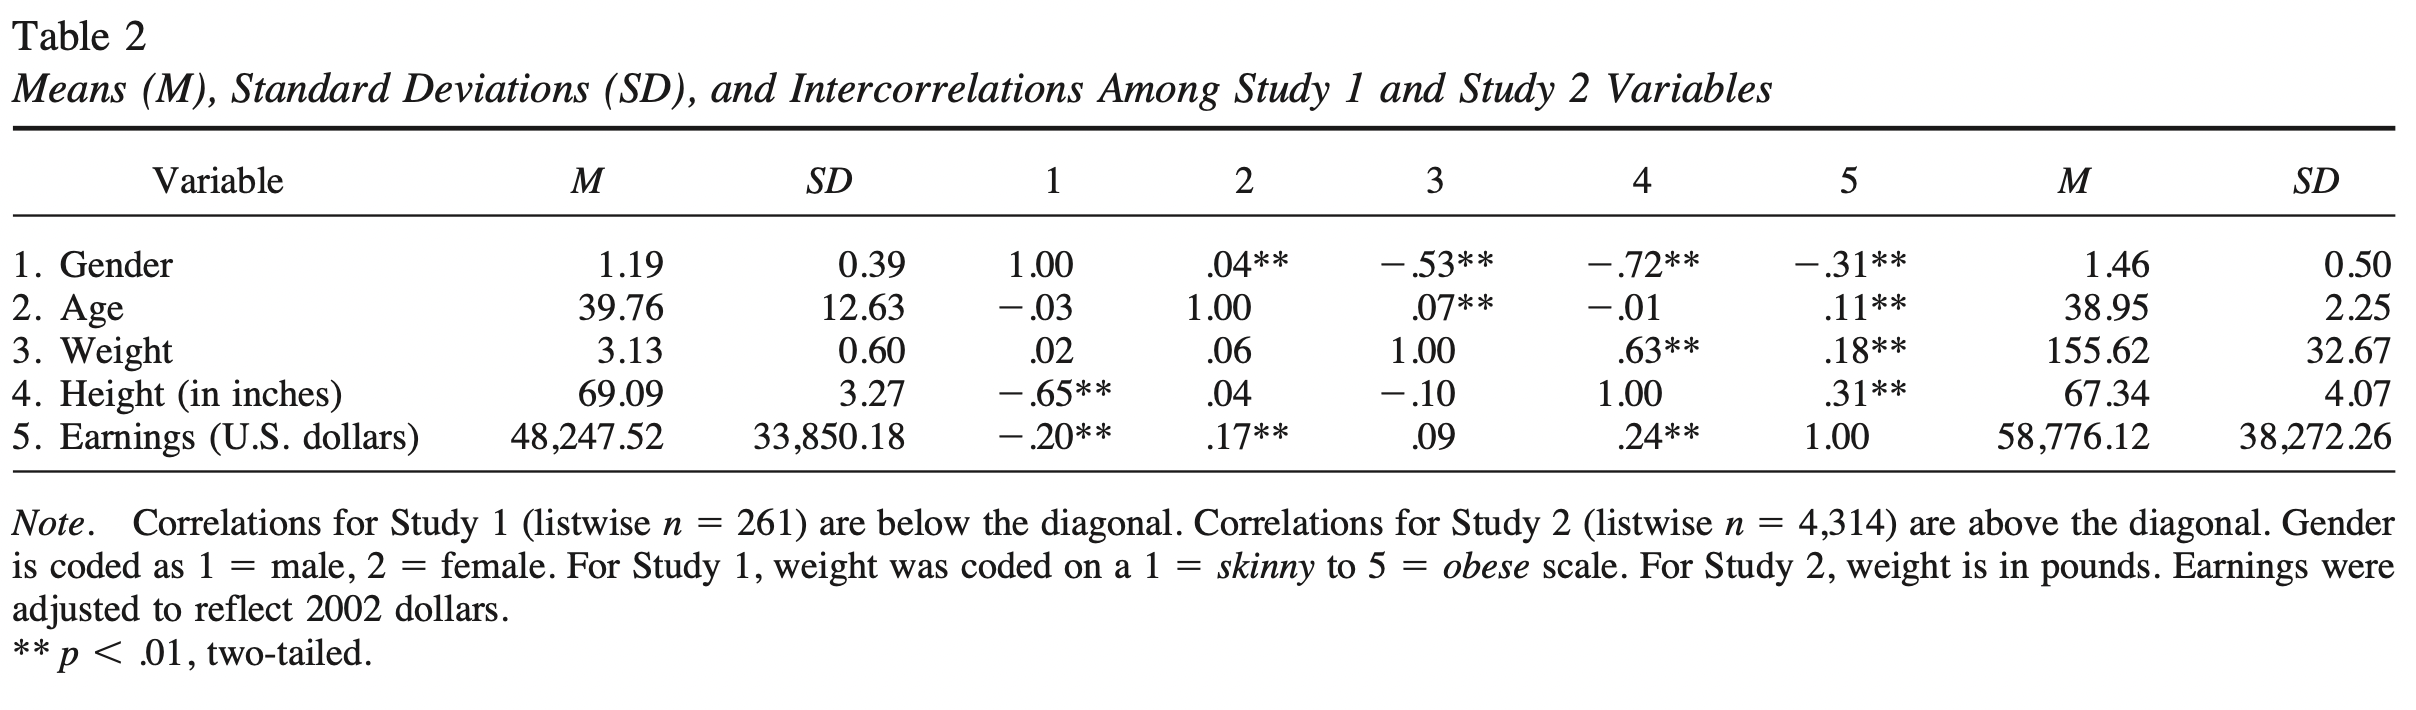
\includegraphics{Skjermbilde 2021-10-21 kl. 10.30.39.png}
\caption{Study 1 and 2}
\end{figure}

\hypertarget{study-3-and-4}{%
\section{\texorpdfstring{\protect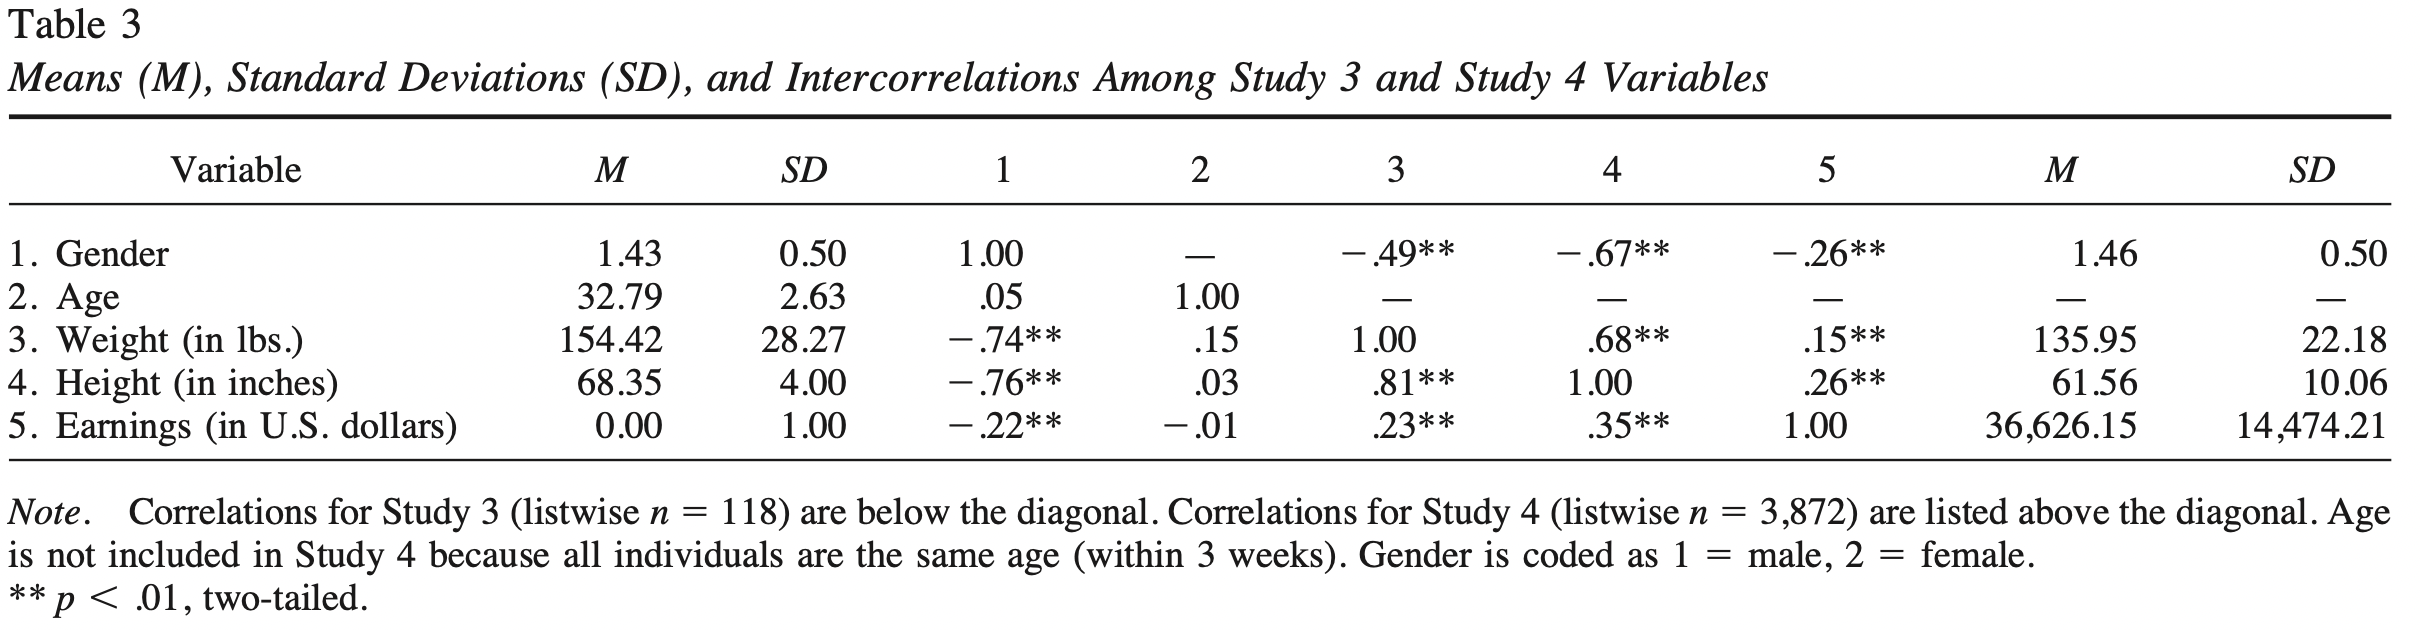
\includegraphics{Skjermbilde 2021-10-21 kl. 10.29.47.png}}{Study 3 and 4}}\label{study-3-and-4}}

\hypertarget{analyse}{%
\subsection{Analyse}\label{analyse}}

\begin{Shaded}
\begin{Highlighting}[]
\NormalTok{hoyde }\OtherTok{\textless{}{-}}\NormalTok{ heights}
\FunctionTok{attach}\NormalTok{(hoyde)}
\end{Highlighting}
\end{Shaded}

Her tar vi å gjør om til målenhetene til metriske. Vi har også lagt til
tre nye variabler.

\begin{Shaded}
\begin{Highlighting}[]
\NormalTok{hoyde }\OtherTok{\textless{}{-}}\NormalTok{ hoyde }\SpecialCharTok{\%\textgreater{}\%} 
  \FunctionTok{mutate}\NormalTok{(}\AttributeTok{inntekt =}\NormalTok{ income }\SpecialCharTok{*} \FloatTok{8.42}\NormalTok{,}
         \AttributeTok{hoyde\_cm =}\NormalTok{ height }\SpecialCharTok{*} \FloatTok{2.54}\NormalTok{,}
         \AttributeTok{vekt\_kg =}\NormalTok{ weight }\SpecialCharTok{*} \FloatTok{0.454}\NormalTok{,}
         \AttributeTok{BMI =}\NormalTok{ vekt\_kg}\SpecialCharTok{/}\NormalTok{(hoyde\_cm}\SpecialCharTok{/}\DecValTok{100}\NormalTok{)}\SpecialCharTok{\^{}}\DecValTok{2}\NormalTok{)}
\end{Highlighting}
\end{Shaded}

\hypertarget{beskrivende-statistikk}{%
\subsubsection{Beskrivende statistikk}\label{beskrivende-statistikk}}

\begin{itemize}
\tightlist
\item
  income: Dette er den årlige inntekten. Her ble topp to prosent av
  inntektene ble gjort om til gjennomsnittet mellom disse og erstatter
  inntektene som er i toppen.
\item
  height: Høyde i tommer
\item
  weight: Vekt i pund
\item
  age: Alder mellom 47 og 56 år.
\item
  marital: Sivilstatus
\item
  sex: Kjønn:
\item
  education: Antall år med utdanning
\item
  afqt: Prosentscore i hvor mye du egner deg i militæret
\end{itemize}

Grunnen til utliggerne ut til høyre er på grunn av personvern under
deltakelsen. Der de høyeste lønningene ble lagt sammen og regnt ut
gjennomsnittet på disse lønningene.

\begin{Shaded}
\begin{Highlighting}[]
\FunctionTok{ggplot}\NormalTok{(hoyde, }\AttributeTok{mapping =} \FunctionTok{aes}\NormalTok{(}\AttributeTok{x =}\NormalTok{ income)) }\SpecialCharTok{+}
  \FunctionTok{geom\_histogram}\NormalTok{()}
\end{Highlighting}
\end{Shaded}

\begin{verbatim}
## `stat_bin()` using `bins = 30`. Pick better value with `binwidth`.
\end{verbatim}

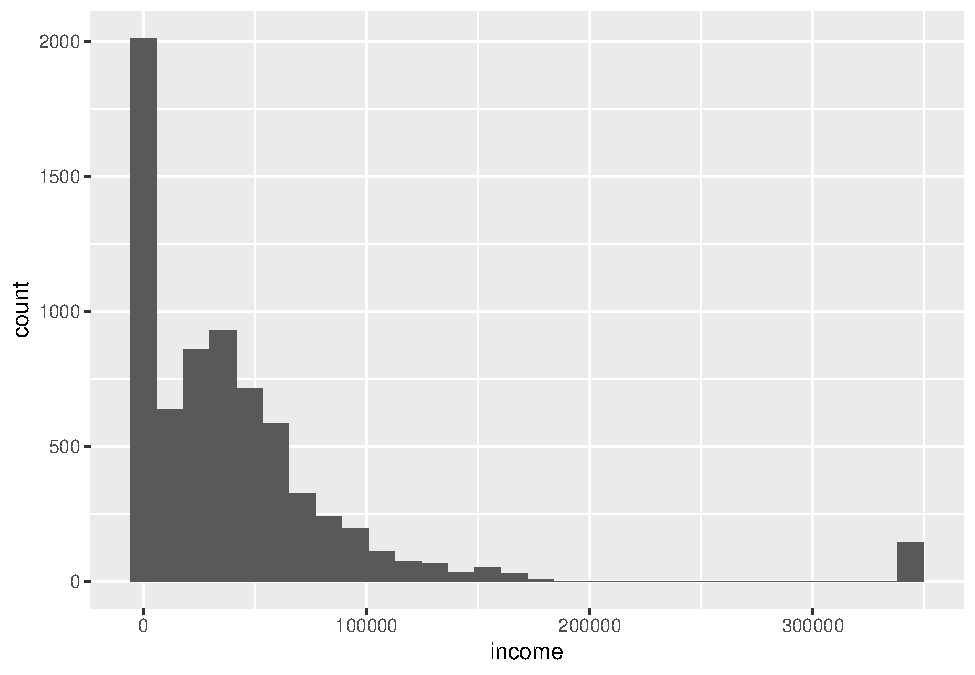
\includegraphics{arbeidskrav2_files/figure-latex/unnamed-chunk-4-1.pdf}

\begin{Shaded}
\begin{Highlighting}[]
  \FunctionTok{geom\_histogram}\NormalTok{(}\AttributeTok{bins =} \DecValTok{30}\NormalTok{)}
\end{Highlighting}
\end{Shaded}

\begin{verbatim}
## geom_bar: na.rm = FALSE, orientation = NA
## stat_bin: binwidth = NULL, bins = 30, na.rm = FALSE, orientation = NA, pad = FALSE
## position_stack
\end{verbatim}

\begin{Shaded}
\begin{Highlighting}[]
\NormalTok{hoyde\_begr }\OtherTok{\textless{}{-}}\NormalTok{ hoyde }\SpecialCharTok{\%\textgreater{}\%} 
  \FunctionTok{filter}\NormalTok{(inntekt }\SpecialCharTok{\textless{}} \DecValTok{1500000}\NormalTok{,}
\NormalTok{         inntekt }\SpecialCharTok{\textgreater{}} \DecValTok{1}\NormalTok{)}
\end{Highlighting}
\end{Shaded}

\hypertarget{exploratory-data-analysis-eda-vha.-ggplot}{%
\subsubsection{Exploratory Data Analysis (EDA) vha.
ggplot}\label{exploratory-data-analysis-eda-vha.-ggplot}}

\begin{Shaded}
\begin{Highlighting}[]
\FunctionTok{ggplot}\NormalTok{(}\AttributeTok{data =}\NormalTok{ hoyde\_begr, }\FunctionTok{aes}\NormalTok{(}\AttributeTok{x =}\NormalTok{ inntekt)) }\SpecialCharTok{+} 
  \FunctionTok{geom\_histogram}\NormalTok{()}
\end{Highlighting}
\end{Shaded}

\begin{verbatim}
## `stat_bin()` using `bins = 30`. Pick better value with `binwidth`.
\end{verbatim}

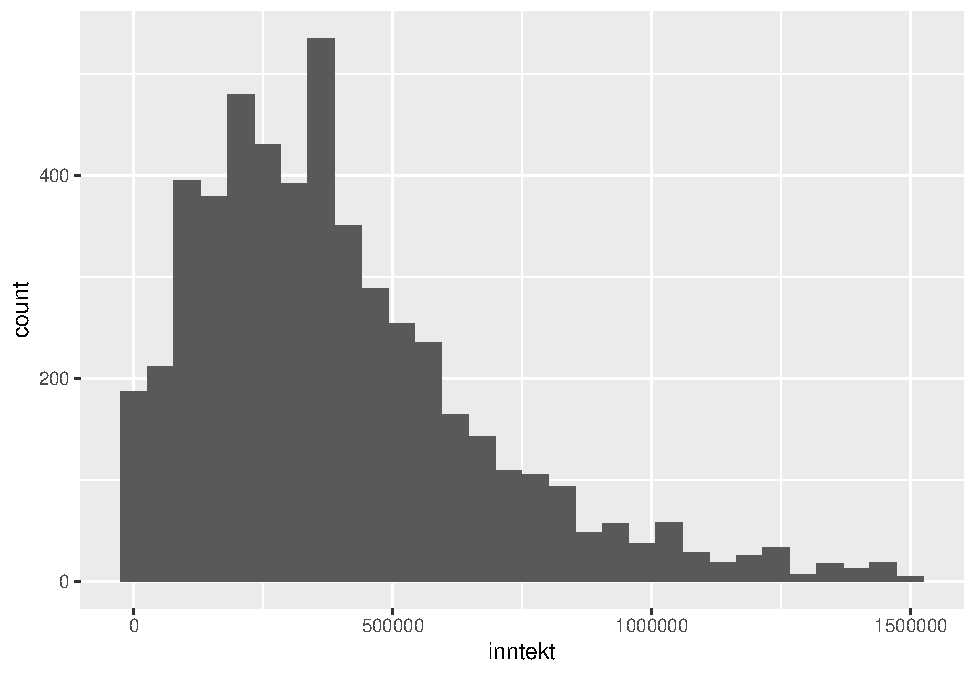
\includegraphics{arbeidskrav2_files/figure-latex/unnamed-chunk-6-1.pdf}

\begin{Shaded}
\begin{Highlighting}[]
\FunctionTok{sum}\NormalTok{(hoyde}\SpecialCharTok{$}\NormalTok{income }\SpecialCharTok{==} \DecValTok{0}\NormalTok{)}
\end{Highlighting}
\end{Shaded}

\begin{verbatim}
## [1] 1740
\end{verbatim}

Det er 1740 personer som står uten inntekt i dette datasettet

\hypertarget{regresjon}{%
\subsection{Regresjon}\label{regresjon}}

\begin{Shaded}
\begin{Highlighting}[]
\NormalTok{mod1 }\OtherTok{\textless{}{-}} \StringTok{"inntekt \textasciitilde{} hoyde\_cm"}
\NormalTok{lm1 }\OtherTok{\textless{}{-}} \FunctionTok{lm}\NormalTok{(mod1, }\AttributeTok{data =}\NormalTok{ hoyde, }\AttributeTok{subset =} \FunctionTok{complete.cases}\NormalTok{(hoyde))}
\end{Highlighting}
\end{Shaded}

\begin{Shaded}
\begin{Highlighting}[]
\FunctionTok{summary}\NormalTok{(lm1)}
\end{Highlighting}
\end{Shaded}

\begin{verbatim}
## 
## Call:
## lm(formula = mod1, data = hoyde, subset = complete.cases(hoyde))
## 
## Residuals:
##     Min      1Q  Median      3Q     Max 
## -782810 -267359  -94513  123099 2699234 
## 
## Coefficients:
##               Estimate Std. Error t value            Pr(>|t|)    
## (Intercept) -1361001.0    94430.0  -14.41 <0.0000000000000002 ***
## hoyde_cm       10047.9      552.8   18.18 <0.0000000000000002 ***
## ---
## Signif. codes:  0 '***' 0.001 '**' 0.01 '*' 0.05 '.' 0.1 ' ' 1
## 
## Residual standard error: 467300 on 6643 degrees of freedom
## Multiple R-squared:  0.04737,    Adjusted R-squared:  0.04723 
## F-statistic: 330.3 on 1 and 6643 DF,  p-value: < 0.00000000000000022
\end{verbatim}

\begin{Shaded}
\begin{Highlighting}[]
\SpecialCharTok{{-}}\DecValTok{1361001} \SpecialCharTok{+}\NormalTok{ (}\FloatTok{10047.9}\SpecialCharTok{*}\DecValTok{162}\NormalTok{)}
\end{Highlighting}
\end{Shaded}

\begin{verbatim}
## [1] 266758.8
\end{verbatim}

\begin{Shaded}
\begin{Highlighting}[]
\SpecialCharTok{{-}}\DecValTok{1361001} \SpecialCharTok{+}\NormalTok{ (}\FloatTok{10047.9}\SpecialCharTok{*}\DecValTok{161}\NormalTok{)}
\end{Highlighting}
\end{Shaded}

\begin{verbatim}
## [1] 256710.9
\end{verbatim}

Vi ser at inntekten vil øke med 10047,9 kr per cm en øker i høyden.

\begin{Shaded}
\begin{Highlighting}[]
\NormalTok{mod2 }\OtherTok{\textless{}{-}} \StringTok{"inntekt \textasciitilde{} hoyde\_cm + vekt\_kg"}
\NormalTok{lm2 }\OtherTok{\textless{}{-}} \FunctionTok{lm}\NormalTok{(mod2, }\AttributeTok{data =}\NormalTok{ hoyde, }\AttributeTok{subset =} \FunctionTok{complete.cases}\NormalTok{(hoyde))}
\end{Highlighting}
\end{Shaded}

\begin{Shaded}
\begin{Highlighting}[]
\FunctionTok{summary}\NormalTok{(lm2)}
\end{Highlighting}
\end{Shaded}

\begin{verbatim}
## 
## Call:
## lm(formula = mod2, data = hoyde, subset = complete.cases(hoyde))
## 
## Residuals:
##     Min      1Q  Median      3Q     Max 
## -843668 -263322  -92573  125798 2715000 
## 
## Coefficients:
##               Estimate Std. Error t value             Pr(>|t|)    
## (Intercept) -1466873.6    96890.5 -15.139 < 0.0000000000000002 ***
## hoyde_cm       11430.3      624.3  18.308 < 0.0000000000000002 ***
## vekt_kg        -1518.4      320.5  -4.737           0.00000221 ***
## ---
## Signif. codes:  0 '***' 0.001 '**' 0.01 '*' 0.05 '.' 0.1 ' ' 1
## 
## Residual standard error: 466600 on 6642 degrees of freedom
## Multiple R-squared:  0.05058,    Adjusted R-squared:  0.05029 
## F-statistic: 176.9 on 2 and 6642 DF,  p-value: < 0.00000000000000022
\end{verbatim}

\begin{Shaded}
\begin{Highlighting}[]
\SpecialCharTok{{-}}\FloatTok{1466873.6} \SpecialCharTok{+}\NormalTok{ (}\FloatTok{11430.3}\SpecialCharTok{*}\DecValTok{162}\NormalTok{) }\SpecialCharTok{+}\NormalTok{ (}\SpecialCharTok{{-}}\FloatTok{1518.4}\SpecialCharTok{*}\DecValTok{62}\NormalTok{)}
\end{Highlighting}
\end{Shaded}

\begin{verbatim}
## [1] 290694.2
\end{verbatim}

\begin{Shaded}
\begin{Highlighting}[]
\SpecialCharTok{{-}}\FloatTok{1466873.6} \SpecialCharTok{+}\NormalTok{ (}\FloatTok{11430.3}\SpecialCharTok{*}\DecValTok{161}\NormalTok{) }\SpecialCharTok{+}\NormalTok{ (}\SpecialCharTok{{-}}\FloatTok{1518.4}\SpecialCharTok{*}\DecValTok{61}\NormalTok{)}
\end{Highlighting}
\end{Shaded}

\begin{verbatim}
## [1] 280782.3
\end{verbatim}

Det vi ser her er at når høyden øker så øker lønnen, men når vekten øker
så gå lønnen ned. En kombinasjon av disse vil gi en økt inntekt.

\begin{Shaded}
\begin{Highlighting}[]
\NormalTok{mod3 }\OtherTok{\textless{}{-}} \StringTok{"inntekt \textasciitilde{} hoyde\_cm + vekt\_kg + BMI"}
\NormalTok{lm3 }\OtherTok{\textless{}{-}} \FunctionTok{lm}\NormalTok{(mod3, }\AttributeTok{data =}\NormalTok{ hoyde, }\AttributeTok{subset =} \FunctionTok{complete.cases}\NormalTok{(hoyde))}
\end{Highlighting}
\end{Shaded}

\begin{Shaded}
\begin{Highlighting}[]
\FunctionTok{summary}\NormalTok{(lm3)}
\end{Highlighting}
\end{Shaded}

\begin{verbatim}
## 
## Call:
## lm(formula = mod3, data = hoyde, subset = complete.cases(hoyde))
## 
## Residuals:
##     Min      1Q  Median      3Q     Max 
## -886295 -261634  -93597  124905 2709981 
## 
## Coefficients:
##             Estimate Std. Error t value     Pr(>|t|)    
## (Intercept) -2015890     447005  -4.510 0.0000066012 ***
## hoyde_cm       14669       2649   5.537 0.0000000319 ***
## vekt_kg        -4723       2567  -1.840       0.0658 .  
## BMI             9224       7332   1.258       0.2084    
## ---
## Signif. codes:  0 '***' 0.001 '**' 0.01 '*' 0.05 '.' 0.1 ' ' 1
## 
## Residual standard error: 466600 on 6641 degrees of freedom
## Multiple R-squared:  0.05081,    Adjusted R-squared:  0.05038 
## F-statistic: 118.5 on 3 and 6641 DF,  p-value: < 0.00000000000000022
\end{verbatim}

\begin{Shaded}
\begin{Highlighting}[]
\NormalTok{hoyde }\OtherTok{\textless{}{-}}\NormalTok{ hoyde }\SpecialCharTok{\%\textgreater{}\%} 
  \FunctionTok{mutate}\NormalTok{(}
    \AttributeTok{married =} \FunctionTok{factor}\NormalTok{(}
      \FunctionTok{case\_when}\NormalTok{(}
\NormalTok{        marital }\SpecialCharTok{==} \StringTok{\textquotesingle{}married\textquotesingle{}} \SpecialCharTok{\textasciitilde{}} \ConstantTok{TRUE}\NormalTok{, }\ConstantTok{TRUE} \SpecialCharTok{\textasciitilde{}} \ConstantTok{FALSE}
\NormalTok{      )}
\NormalTok{    )}
\NormalTok{  )}
\end{Highlighting}
\end{Shaded}

\begin{Shaded}
\begin{Highlighting}[]
\FunctionTok{huxreg}\NormalTok{(}
   \FunctionTok{list}\NormalTok{(}\StringTok{"mod1"} \OtherTok{=}\NormalTok{ lm1, }\StringTok{"mod2"} \OtherTok{=}\NormalTok{ lm2, }\StringTok{"mod3"} \OtherTok{=}\NormalTok{ lm3),}
   \AttributeTok{error\_format =} \StringTok{"[\{statistic\}]"}\NormalTok{,}
   \AttributeTok{note =} \StringTok{"Regresjonstabell 3: \{stars\}. T statistics in brackets."}
\NormalTok{   )}
\end{Highlighting}
\end{Shaded}

 
  \providecommand{\huxb}[2]{\arrayrulecolor[RGB]{#1}\global\arrayrulewidth=#2pt}
  \providecommand{\huxvb}[2]{\color[RGB]{#1}\vrule width #2pt}
  \providecommand{\huxtpad}[1]{\rule{0pt}{#1}}
  \providecommand{\huxbpad}[1]{\rule[-#1]{0pt}{#1}}

\begin{table}[ht]
\begin{centerbox}
\begin{threeparttable}
 \label{tab:unnamed-chunk-17}
\setlength{\tabcolsep}{0pt}
\begin{tabular}{l l l l}


\hhline{>{\huxb{0, 0, 0}{0.8}}->{\huxb{0, 0, 0}{0.8}}->{\huxb{0, 0, 0}{0.8}}->{\huxb{0, 0, 0}{0.8}}-}
\arrayrulecolor{black}

\multicolumn{1}{!{\huxvb{0, 0, 0}{0}}c!{\huxvb{0, 0, 0}{0}}}{\huxtpad{6pt + 1em}\centering \hspace{6pt}  \hspace{6pt}\huxbpad{6pt}} &
\multicolumn{1}{c!{\huxvb{0, 0, 0}{0}}}{\huxtpad{6pt + 1em}\centering \hspace{6pt} mod1 \hspace{6pt}\huxbpad{6pt}} &
\multicolumn{1}{c!{\huxvb{0, 0, 0}{0}}}{\huxtpad{6pt + 1em}\centering \hspace{6pt} mod2 \hspace{6pt}\huxbpad{6pt}} &
\multicolumn{1}{c!{\huxvb{0, 0, 0}{0}}}{\huxtpad{6pt + 1em}\centering \hspace{6pt} mod3 \hspace{6pt}\huxbpad{6pt}} \tabularnewline[-0.5pt]


\hhline{>{\huxb{255, 255, 255}{0.4}}->{\huxb{0, 0, 0}{0.4}}->{\huxb{0, 0, 0}{0.4}}->{\huxb{0, 0, 0}{0.4}}-}
\arrayrulecolor{black}

\multicolumn{1}{!{\huxvb{0, 0, 0}{0}}l!{\huxvb{0, 0, 0}{0}}}{\huxtpad{6pt + 1em}\raggedright \hspace{6pt} (Intercept) \hspace{6pt}\huxbpad{6pt}} &
\multicolumn{1}{r!{\huxvb{0, 0, 0}{0}}}{\huxtpad{6pt + 1em}\raggedleft \hspace{6pt} -1361000.990 *** \hspace{6pt}\huxbpad{6pt}} &
\multicolumn{1}{r!{\huxvb{0, 0, 0}{0}}}{\huxtpad{6pt + 1em}\raggedleft \hspace{6pt} -1466873.555 *** \hspace{6pt}\huxbpad{6pt}} &
\multicolumn{1}{r!{\huxvb{0, 0, 0}{0}}}{\huxtpad{6pt + 1em}\raggedleft \hspace{6pt} -2015889.845 *** \hspace{6pt}\huxbpad{6pt}} \tabularnewline[-0.5pt]


\hhline{}
\arrayrulecolor{black}

\multicolumn{1}{!{\huxvb{0, 0, 0}{0}}l!{\huxvb{0, 0, 0}{0}}}{\huxtpad{6pt + 1em}\raggedright \hspace{6pt}  \hspace{6pt}\huxbpad{6pt}} &
\multicolumn{1}{r!{\huxvb{0, 0, 0}{0}}}{\huxtpad{6pt + 1em}\raggedleft \hspace{6pt} [-14.413]\hphantom{0}\hphantom{0}\hphantom{0} \hspace{6pt}\huxbpad{6pt}} &
\multicolumn{1}{r!{\huxvb{0, 0, 0}{0}}}{\huxtpad{6pt + 1em}\raggedleft \hspace{6pt} [-15.139]\hphantom{0}\hphantom{0}\hphantom{0} \hspace{6pt}\huxbpad{6pt}} &
\multicolumn{1}{r!{\huxvb{0, 0, 0}{0}}}{\huxtpad{6pt + 1em}\raggedleft \hspace{6pt} [-4.510]\hphantom{0}\hphantom{0}\hphantom{0} \hspace{6pt}\huxbpad{6pt}} \tabularnewline[-0.5pt]


\hhline{}
\arrayrulecolor{black}

\multicolumn{1}{!{\huxvb{0, 0, 0}{0}}l!{\huxvb{0, 0, 0}{0}}}{\huxtpad{6pt + 1em}\raggedright \hspace{6pt} hoyde\_cm \hspace{6pt}\huxbpad{6pt}} &
\multicolumn{1}{r!{\huxvb{0, 0, 0}{0}}}{\huxtpad{6pt + 1em}\raggedleft \hspace{6pt} 10047.860 *** \hspace{6pt}\huxbpad{6pt}} &
\multicolumn{1}{r!{\huxvb{0, 0, 0}{0}}}{\huxtpad{6pt + 1em}\raggedleft \hspace{6pt} 11430.259 *** \hspace{6pt}\huxbpad{6pt}} &
\multicolumn{1}{r!{\huxvb{0, 0, 0}{0}}}{\huxtpad{6pt + 1em}\raggedleft \hspace{6pt} 14669.413 *** \hspace{6pt}\huxbpad{6pt}} \tabularnewline[-0.5pt]


\hhline{}
\arrayrulecolor{black}

\multicolumn{1}{!{\huxvb{0, 0, 0}{0}}l!{\huxvb{0, 0, 0}{0}}}{\huxtpad{6pt + 1em}\raggedright \hspace{6pt}  \hspace{6pt}\huxbpad{6pt}} &
\multicolumn{1}{r!{\huxvb{0, 0, 0}{0}}}{\huxtpad{6pt + 1em}\raggedleft \hspace{6pt} [18.175]\hphantom{0}\hphantom{0}\hphantom{0} \hspace{6pt}\huxbpad{6pt}} &
\multicolumn{1}{r!{\huxvb{0, 0, 0}{0}}}{\huxtpad{6pt + 1em}\raggedleft \hspace{6pt} [18.308]\hphantom{0}\hphantom{0}\hphantom{0} \hspace{6pt}\huxbpad{6pt}} &
\multicolumn{1}{r!{\huxvb{0, 0, 0}{0}}}{\huxtpad{6pt + 1em}\raggedleft \hspace{6pt} [5.537]\hphantom{0}\hphantom{0}\hphantom{0} \hspace{6pt}\huxbpad{6pt}} \tabularnewline[-0.5pt]


\hhline{}
\arrayrulecolor{black}

\multicolumn{1}{!{\huxvb{0, 0, 0}{0}}l!{\huxvb{0, 0, 0}{0}}}{\huxtpad{6pt + 1em}\raggedright \hspace{6pt} vekt\_kg \hspace{6pt}\huxbpad{6pt}} &
\multicolumn{1}{r!{\huxvb{0, 0, 0}{0}}}{\huxtpad{6pt + 1em}\raggedleft \hspace{6pt} \hphantom{0}\hphantom{0}\hphantom{0}\hphantom{0}\hphantom{0}\hphantom{0}\hphantom{0}\hphantom{0} \hspace{6pt}\huxbpad{6pt}} &
\multicolumn{1}{r!{\huxvb{0, 0, 0}{0}}}{\huxtpad{6pt + 1em}\raggedleft \hspace{6pt} -1518.381 *** \hspace{6pt}\huxbpad{6pt}} &
\multicolumn{1}{r!{\huxvb{0, 0, 0}{0}}}{\huxtpad{6pt + 1em}\raggedleft \hspace{6pt} -4722.577\hphantom{0}\hphantom{0}\hphantom{0}\hphantom{0} \hspace{6pt}\huxbpad{6pt}} \tabularnewline[-0.5pt]


\hhline{}
\arrayrulecolor{black}

\multicolumn{1}{!{\huxvb{0, 0, 0}{0}}l!{\huxvb{0, 0, 0}{0}}}{\huxtpad{6pt + 1em}\raggedright \hspace{6pt}  \hspace{6pt}\huxbpad{6pt}} &
\multicolumn{1}{r!{\huxvb{0, 0, 0}{0}}}{\huxtpad{6pt + 1em}\raggedleft \hspace{6pt} \hphantom{0}\hphantom{0}\hphantom{0}\hphantom{0}\hphantom{0}\hphantom{0}\hphantom{0}\hphantom{0} \hspace{6pt}\huxbpad{6pt}} &
\multicolumn{1}{r!{\huxvb{0, 0, 0}{0}}}{\huxtpad{6pt + 1em}\raggedleft \hspace{6pt} [-4.737]\hphantom{0}\hphantom{0}\hphantom{0} \hspace{6pt}\huxbpad{6pt}} &
\multicolumn{1}{r!{\huxvb{0, 0, 0}{0}}}{\huxtpad{6pt + 1em}\raggedleft \hspace{6pt} [-1.840]\hphantom{0}\hphantom{0}\hphantom{0} \hspace{6pt}\huxbpad{6pt}} \tabularnewline[-0.5pt]


\hhline{}
\arrayrulecolor{black}

\multicolumn{1}{!{\huxvb{0, 0, 0}{0}}l!{\huxvb{0, 0, 0}{0}}}{\huxtpad{6pt + 1em}\raggedright \hspace{6pt} BMI \hspace{6pt}\huxbpad{6pt}} &
\multicolumn{1}{r!{\huxvb{0, 0, 0}{0}}}{\huxtpad{6pt + 1em}\raggedleft \hspace{6pt} \hphantom{0}\hphantom{0}\hphantom{0}\hphantom{0}\hphantom{0}\hphantom{0}\hphantom{0}\hphantom{0} \hspace{6pt}\huxbpad{6pt}} &
\multicolumn{1}{r!{\huxvb{0, 0, 0}{0}}}{\huxtpad{6pt + 1em}\raggedleft \hspace{6pt} \hphantom{0}\hphantom{0}\hphantom{0}\hphantom{0}\hphantom{0}\hphantom{0}\hphantom{0}\hphantom{0} \hspace{6pt}\huxbpad{6pt}} &
\multicolumn{1}{r!{\huxvb{0, 0, 0}{0}}}{\huxtpad{6pt + 1em}\raggedleft \hspace{6pt} 9224.408\hphantom{0}\hphantom{0}\hphantom{0}\hphantom{0} \hspace{6pt}\huxbpad{6pt}} \tabularnewline[-0.5pt]


\hhline{}
\arrayrulecolor{black}

\multicolumn{1}{!{\huxvb{0, 0, 0}{0}}l!{\huxvb{0, 0, 0}{0}}}{\huxtpad{6pt + 1em}\raggedright \hspace{6pt}  \hspace{6pt}\huxbpad{6pt}} &
\multicolumn{1}{r!{\huxvb{0, 0, 0}{0}}}{\huxtpad{6pt + 1em}\raggedleft \hspace{6pt} \hphantom{0}\hphantom{0}\hphantom{0}\hphantom{0}\hphantom{0}\hphantom{0}\hphantom{0}\hphantom{0} \hspace{6pt}\huxbpad{6pt}} &
\multicolumn{1}{r!{\huxvb{0, 0, 0}{0}}}{\huxtpad{6pt + 1em}\raggedleft \hspace{6pt} \hphantom{0}\hphantom{0}\hphantom{0}\hphantom{0}\hphantom{0}\hphantom{0}\hphantom{0}\hphantom{0} \hspace{6pt}\huxbpad{6pt}} &
\multicolumn{1}{r!{\huxvb{0, 0, 0}{0}}}{\huxtpad{6pt + 1em}\raggedleft \hspace{6pt} [1.258]\hphantom{0}\hphantom{0}\hphantom{0} \hspace{6pt}\huxbpad{6pt}} \tabularnewline[-0.5pt]


\hhline{>{\huxb{255, 255, 255}{0.4}}->{\huxb{0, 0, 0}{0.4}}->{\huxb{0, 0, 0}{0.4}}->{\huxb{0, 0, 0}{0.4}}-}
\arrayrulecolor{black}

\multicolumn{1}{!{\huxvb{0, 0, 0}{0}}l!{\huxvb{0, 0, 0}{0}}}{\huxtpad{6pt + 1em}\raggedright \hspace{6pt} N \hspace{6pt}\huxbpad{6pt}} &
\multicolumn{1}{r!{\huxvb{0, 0, 0}{0}}}{\huxtpad{6pt + 1em}\raggedleft \hspace{6pt} 6645\hphantom{0}\hphantom{0}\hphantom{0}\hphantom{0}\hphantom{0}\hphantom{0}\hphantom{0}\hphantom{0} \hspace{6pt}\huxbpad{6pt}} &
\multicolumn{1}{r!{\huxvb{0, 0, 0}{0}}}{\huxtpad{6pt + 1em}\raggedleft \hspace{6pt} 6645\hphantom{0}\hphantom{0}\hphantom{0}\hphantom{0}\hphantom{0}\hphantom{0}\hphantom{0}\hphantom{0} \hspace{6pt}\huxbpad{6pt}} &
\multicolumn{1}{r!{\huxvb{0, 0, 0}{0}}}{\huxtpad{6pt + 1em}\raggedleft \hspace{6pt} 6645\hphantom{0}\hphantom{0}\hphantom{0}\hphantom{0}\hphantom{0}\hphantom{0}\hphantom{0}\hphantom{0} \hspace{6pt}\huxbpad{6pt}} \tabularnewline[-0.5pt]


\hhline{}
\arrayrulecolor{black}

\multicolumn{1}{!{\huxvb{0, 0, 0}{0}}l!{\huxvb{0, 0, 0}{0}}}{\huxtpad{6pt + 1em}\raggedright \hspace{6pt} R2 \hspace{6pt}\huxbpad{6pt}} &
\multicolumn{1}{r!{\huxvb{0, 0, 0}{0}}}{\huxtpad{6pt + 1em}\raggedleft \hspace{6pt} 0.047\hphantom{0}\hphantom{0}\hphantom{0}\hphantom{0} \hspace{6pt}\huxbpad{6pt}} &
\multicolumn{1}{r!{\huxvb{0, 0, 0}{0}}}{\huxtpad{6pt + 1em}\raggedleft \hspace{6pt} 0.051\hphantom{0}\hphantom{0}\hphantom{0}\hphantom{0} \hspace{6pt}\huxbpad{6pt}} &
\multicolumn{1}{r!{\huxvb{0, 0, 0}{0}}}{\huxtpad{6pt + 1em}\raggedleft \hspace{6pt} 0.051\hphantom{0}\hphantom{0}\hphantom{0}\hphantom{0} \hspace{6pt}\huxbpad{6pt}} \tabularnewline[-0.5pt]


\hhline{}
\arrayrulecolor{black}

\multicolumn{1}{!{\huxvb{0, 0, 0}{0}}l!{\huxvb{0, 0, 0}{0}}}{\huxtpad{6pt + 1em}\raggedright \hspace{6pt} logLik \hspace{6pt}\huxbpad{6pt}} &
\multicolumn{1}{r!{\huxvb{0, 0, 0}{0}}}{\huxtpad{6pt + 1em}\raggedleft \hspace{6pt} -96177.211\hphantom{0}\hphantom{0}\hphantom{0}\hphantom{0} \hspace{6pt}\huxbpad{6pt}} &
\multicolumn{1}{r!{\huxvb{0, 0, 0}{0}}}{\huxtpad{6pt + 1em}\raggedleft \hspace{6pt} -96166.004\hphantom{0}\hphantom{0}\hphantom{0}\hphantom{0} \hspace{6pt}\huxbpad{6pt}} &
\multicolumn{1}{r!{\huxvb{0, 0, 0}{0}}}{\huxtpad{6pt + 1em}\raggedleft \hspace{6pt} -96165.212\hphantom{0}\hphantom{0}\hphantom{0}\hphantom{0} \hspace{6pt}\huxbpad{6pt}} \tabularnewline[-0.5pt]


\hhline{}
\arrayrulecolor{black}

\multicolumn{1}{!{\huxvb{0, 0, 0}{0}}l!{\huxvb{0, 0, 0}{0}}}{\huxtpad{6pt + 1em}\raggedright \hspace{6pt} AIC \hspace{6pt}\huxbpad{6pt}} &
\multicolumn{1}{r!{\huxvb{0, 0, 0}{0}}}{\huxtpad{6pt + 1em}\raggedleft \hspace{6pt} 192360.423\hphantom{0}\hphantom{0}\hphantom{0}\hphantom{0} \hspace{6pt}\huxbpad{6pt}} &
\multicolumn{1}{r!{\huxvb{0, 0, 0}{0}}}{\huxtpad{6pt + 1em}\raggedleft \hspace{6pt} 192340.008\hphantom{0}\hphantom{0}\hphantom{0}\hphantom{0} \hspace{6pt}\huxbpad{6pt}} &
\multicolumn{1}{r!{\huxvb{0, 0, 0}{0}}}{\huxtpad{6pt + 1em}\raggedleft \hspace{6pt} 192340.424\hphantom{0}\hphantom{0}\hphantom{0}\hphantom{0} \hspace{6pt}\huxbpad{6pt}} \tabularnewline[-0.5pt]


\hhline{>{\huxb{0, 0, 0}{0.8}}->{\huxb{0, 0, 0}{0.8}}->{\huxb{0, 0, 0}{0.8}}->{\huxb{0, 0, 0}{0.8}}-}
\arrayrulecolor{black}

\multicolumn{4}{!{\huxvb{0, 0, 0}{0}}l!{\huxvb{0, 0, 0}{0}}}{\huxtpad{6pt + 1em}\raggedright \hspace{6pt} Regresjonstabell 3:  *** p $<$ 0.001;  ** p $<$ 0.01;  * p $<$ 0.05. T statistics in brackets. \hspace{6pt}\huxbpad{6pt}} \tabularnewline[-0.5pt]


\hhline{}
\arrayrulecolor{black}
\end{tabular}
\end{threeparttable}\par\end{centerbox}

\end{table}
 

\hypertarget{interaksjon}{%
\subsubsection{interaksjon}\label{interaksjon}}

\begin{Shaded}
\begin{Highlighting}[]
\NormalTok{mod4 }\OtherTok{\textless{}{-}} \StringTok{"inntekt \textasciitilde{} sex*(hoyde\_cm + vekt\_kg + I(vekt\_kg\^{}2)) + BMI + I(BMI\^{}2)"}
\NormalTok{lm4 }\OtherTok{\textless{}{-}} \FunctionTok{lm}\NormalTok{(mod4, }\AttributeTok{data =}\NormalTok{ hoyde)}
\FunctionTok{summary}\NormalTok{(lm4)}
\end{Highlighting}
\end{Shaded}

\begin{verbatim}
## 
## Call:
## lm(formula = mod4, data = hoyde)
## 
## Residuals:
##     Min      1Q  Median      3Q     Max 
## -864444 -245100  -91019  126362 2681172 
## 
## Coefficients:
##                           Estimate  Std. Error t value  Pr(>|t|)    
## (Intercept)            -2821666.91  1904365.52  -1.482   0.13847    
## sexfemale               1181398.44   293082.63   4.031 0.0000562 ***
## hoyde_cm                  17091.78    10627.73   1.608   0.10783    
## vekt_kg                   -4749.34    17977.28  -0.264   0.79164    
## I(vekt_kg^2)                -17.95       42.26  -0.425   0.67109    
## BMI                       34177.41    57584.98   0.594   0.55286    
## I(BMI^2)                   -190.52      435.11  -0.438   0.66150    
## sexfemale:hoyde_cm        -4729.20     1812.91  -2.609   0.00911 ** 
## sexfemale:vekt_kg         -9825.85     5200.88  -1.889   0.05890 .  
## sexfemale:I(vekt_kg^2)       45.96       27.06   1.699   0.08941 .  
## ---
## Signif. codes:  0 '***' 0.001 '**' 0.01 '*' 0.05 '.' 0.1 ' ' 1
## 
## Residual standard error: 458300 on 6901 degrees of freedom
##   (95 observations deleted due to missingness)
## Multiple R-squared:  0.06165,    Adjusted R-squared:  0.06043 
## F-statistic: 50.38 on 9 and 6901 DF,  p-value: < 0.00000000000000022
\end{verbatim}

\begin{Shaded}
\begin{Highlighting}[]
 \FunctionTok{linearHypothesis}\NormalTok{(lm4, }\FunctionTok{c}\NormalTok{(}\StringTok{"sexfemale = 0"}\NormalTok{, }\StringTok{"sexfemale:hoyde\_cm = 0"}\NormalTok{))}
\end{Highlighting}
\end{Shaded}

 
  \providecommand{\huxb}[2]{\arrayrulecolor[RGB]{#1}\global\arrayrulewidth=#2pt}
  \providecommand{\huxvb}[2]{\color[RGB]{#1}\vrule width #2pt}
  \providecommand{\huxtpad}[1]{\rule{0pt}{#1}}
  \providecommand{\huxbpad}[1]{\rule[-#1]{0pt}{#1}}

\begin{table}[ht]
\begin{centerbox}
\begin{threeparttable}
 \label{tab:unnamed-chunk-19}
\setlength{\tabcolsep}{0pt}
\begin{tabular}{l l l l l l}


\hhline{>{\huxb{0, 0, 0}{0.4}}->{\huxb{0, 0, 0}{0.4}}->{\huxb{0, 0, 0}{0.4}}->{\huxb{0, 0, 0}{0.4}}->{\huxb{0, 0, 0}{0.4}}->{\huxb{0, 0, 0}{0.4}}-}
\arrayrulecolor{black}

\multicolumn{1}{!{\huxvb{0, 0, 0}{0.4}}r!{\huxvb{0, 0, 0}{0}}}{\huxtpad{6pt + 1em}\raggedleft \hspace{6pt} \textbf{Res.Df} \hspace{6pt}\huxbpad{6pt}} &
\multicolumn{1}{r!{\huxvb{0, 0, 0}{0}}}{\huxtpad{6pt + 1em}\raggedleft \hspace{6pt} \textbf{RSS} \hspace{6pt}\huxbpad{6pt}} &
\multicolumn{1}{r!{\huxvb{0, 0, 0}{0}}}{\huxtpad{6pt + 1em}\raggedleft \hspace{6pt} \textbf{Df} \hspace{6pt}\huxbpad{6pt}} &
\multicolumn{1}{r!{\huxvb{0, 0, 0}{0}}}{\huxtpad{6pt + 1em}\raggedleft \hspace{6pt} \textbf{Sum of Sq} \hspace{6pt}\huxbpad{6pt}} &
\multicolumn{1}{r!{\huxvb{0, 0, 0}{0}}}{\huxtpad{6pt + 1em}\raggedleft \hspace{6pt} \textbf{F} \hspace{6pt}\huxbpad{6pt}} &
\multicolumn{1}{r!{\huxvb{0, 0, 0}{0.4}}}{\huxtpad{6pt + 1em}\raggedleft \hspace{6pt} \textbf{Pr($>$F)} \hspace{6pt}\huxbpad{6pt}} \tabularnewline[-0.5pt]


\hhline{>{\huxb{0, 0, 0}{0.4}}->{\huxb{0, 0, 0}{0.4}}->{\huxb{0, 0, 0}{0.4}}->{\huxb{0, 0, 0}{0.4}}->{\huxb{0, 0, 0}{0.4}}->{\huxb{0, 0, 0}{0.4}}-}
\arrayrulecolor{black}

\multicolumn{1}{!{\huxvb{0, 0, 0}{0.4}}r!{\huxvb{0, 0, 0}{0}}}{\cellcolor[RGB]{242, 242, 242}\huxtpad{6pt + 1em}\raggedleft \hspace{6pt} 6.9e+03 \hspace{6pt}\huxbpad{6pt}} &
\multicolumn{1}{r!{\huxvb{0, 0, 0}{0}}}{\cellcolor[RGB]{242, 242, 242}\huxtpad{6pt + 1em}\raggedleft \hspace{6pt} 1.45e+15 \hspace{6pt}\huxbpad{6pt}} &
\multicolumn{1}{r!{\huxvb{0, 0, 0}{0}}}{\cellcolor[RGB]{242, 242, 242}\huxtpad{6pt + 1em}\raggedleft \hspace{6pt}  \hspace{6pt}\huxbpad{6pt}} &
\multicolumn{1}{r!{\huxvb{0, 0, 0}{0}}}{\cellcolor[RGB]{242, 242, 242}\huxtpad{6pt + 1em}\raggedleft \hspace{6pt} \hphantom{0}\hphantom{0}\hphantom{0}\hphantom{0}\hphantom{0}\hphantom{0}\hphantom{0} \hspace{6pt}\huxbpad{6pt}} &
\multicolumn{1}{r!{\huxvb{0, 0, 0}{0}}}{\cellcolor[RGB]{242, 242, 242}\huxtpad{6pt + 1em}\raggedleft \hspace{6pt} \hphantom{0}\hphantom{0}\hphantom{0} \hspace{6pt}\huxbpad{6pt}} &
\multicolumn{1}{r!{\huxvb{0, 0, 0}{0.4}}}{\cellcolor[RGB]{242, 242, 242}\huxtpad{6pt + 1em}\raggedleft \hspace{6pt} \hphantom{0}\hphantom{0}\hphantom{0}\hphantom{0}\hphantom{0}\hphantom{0}\hphantom{0} \hspace{6pt}\huxbpad{6pt}} \tabularnewline[-0.5pt]


\hhline{>{\huxb{0, 0, 0}{0.4}}|>{\huxb{0, 0, 0}{0.4}}|}
\arrayrulecolor{black}

\multicolumn{1}{!{\huxvb{0, 0, 0}{0.4}}r!{\huxvb{0, 0, 0}{0}}}{\huxtpad{6pt + 1em}\raggedleft \hspace{6pt} 6.9e+03 \hspace{6pt}\huxbpad{6pt}} &
\multicolumn{1}{r!{\huxvb{0, 0, 0}{0}}}{\huxtpad{6pt + 1em}\raggedleft \hspace{6pt} 1.45e+15 \hspace{6pt}\huxbpad{6pt}} &
\multicolumn{1}{r!{\huxvb{0, 0, 0}{0}}}{\huxtpad{6pt + 1em}\raggedleft \hspace{6pt} 2 \hspace{6pt}\huxbpad{6pt}} &
\multicolumn{1}{r!{\huxvb{0, 0, 0}{0}}}{\huxtpad{6pt + 1em}\raggedleft \hspace{6pt} 3.42e+12 \hspace{6pt}\huxbpad{6pt}} &
\multicolumn{1}{r!{\huxvb{0, 0, 0}{0}}}{\huxtpad{6pt + 1em}\raggedleft \hspace{6pt} 8.13 \hspace{6pt}\huxbpad{6pt}} &
\multicolumn{1}{r!{\huxvb{0, 0, 0}{0.4}}}{\huxtpad{6pt + 1em}\raggedleft \hspace{6pt} 0.000297 \hspace{6pt}\huxbpad{6pt}} \tabularnewline[-0.5pt]


\hhline{>{\huxb{0, 0, 0}{0.4}}->{\huxb{0, 0, 0}{0.4}}->{\huxb{0, 0, 0}{0.4}}->{\huxb{0, 0, 0}{0.4}}->{\huxb{0, 0, 0}{0.4}}->{\huxb{0, 0, 0}{0.4}}-}
\arrayrulecolor{black}
\end{tabular}
\end{threeparttable}\par\end{centerbox}

\end{table}
 

\end{document}
